\documentclass[11pt,a4paper]{article}

\usepackage[margin=2.5cm]{geometry}
\usepackage{amsmath,amssymb,amsthm}
\usepackage{booktabs}
\usepackage{siunitx}
\usepackage{pgfplots}
\usepackage{caption}
\usepackage[hidelinks]{hyperref}
\usepackage{microtype}

\pgfplotsset{compat=1.17}
\sisetup{group-digits=integer}

\theoremstyle{plain}
\newtheorem{proposition}{Proposition}
\newtheorem{lemma}[proposition]{Lemma}
\theoremstyle{definition}
\newtheorem{definition}[proposition]{Definition}
\theoremstyle{remark}
\newtheorem{remark}[proposition]{Remark}

\newcommand{\FF}{\mathbb{F}}
\newcommand{\QQ}{\mathbb{Q}}
\newcommand{\CC}{\mathbb{C}}
\newcommand{\Aff}{\mathbb{A}}
\newcommand{\bp}{\boldsymbol{p}}
\newcommand{\bt}{\boldsymbol{t}}
\newcommand{\In}{\operatorname{in}}
\newcommand{\LM}{\operatorname{LM}}

\title{\bfseries The cost of parametric Gr\"obner basis computation\\ over a rational function field}
\author{Haniel Ulises}
\date{5 September 2026}

\begin{document}
\maketitle

\begin{abstract}
\noindent
Inverse kinematics can be posed so that the target pose is adjoined to the coefficient field rather
than substituted into the polynomial ring. A single Gr\"obner basis over $\QQ(\bp)$ then answers
every pose, which is what permits an offline solve and generated runtime code. In the implementation
studied here this computation completes in milliseconds with two adjoined parameters and has not been
observed to complete with three. Profiling attributes approximately \SI{86}{\percent} of the running
time to the polynomial greatest common divisor invoked when coefficients are reduced to lowest terms,
which suggests that a modular gcd would remove the limitation. We test that suggestion by repeating
the computation over $\FF_p(\bp)$, where coefficient arithmetic is a single machine-word operation
and coefficients do not grow. The three-parameter problem fails to terminate over $\FF_p$ as well.
An independent measurement of the subresultant gcd over both fields, on dense trivariate operands
ranging from $35$ to $969$ terms, gives fitted cost exponents of $3.79$ over $\FF_p$ and $3.81$ over
$\QQ$, with a ratio between the fields that rises to and settles near $13$. The choice of coefficient
field therefore governs a bounded multiplicative constant while the growth in operand size governs
the exponent. Since the operands reached during a single reduction of the three-parameter run number
$498$ terms, a value interior to the measured range, we conclude that a modular gcd formed by
computing the existing remainder sequence over several primes cannot make the problem tractable, and
that only a gcd based on evaluation and interpolation addresses the measured cost.
\end{abstract}

\section{Introduction}
\label{sec:introduction}

The inverse kinematics of a serial manipulator with revolute joints becomes a polynomial system under
the tangent half-angle substitution $t_i = \tan(q_i/2)$, and the resulting zero-dimensional ideal can
be solved by the eigenvalue method of M\"oller and Stetter~\cite{moller1995}. Classical treatments of
the general $6R$ arm reduce the problem to a univariate resultant of degree
sixteen~\cite{leeliang1988,raghavanroth1993,manochacanny1994}. The system studied here takes a
different route: the target pose is adjoined to the coefficient field, so that the Gr\"obner basis is
computed once for the manipulator and evaluated at each requested pose, and the action matrices of
the quotient algebra are emitted as source code.

The cost of this formulation is the subject of the present report. Writing $N$ for the number of
actuated joints and $P$ for the number of adjoined pose coordinates, the observed behaviour of the
implementation is
\begin{itemize}
  \item $P = N = 2$: complete in \SIrange{6}{33}{\milli\second};
  \item $P = N = 3$: no result after \SI{900}{\second}.
\end{itemize}
An instrumented run of the three-parameter problem attributes approximately \SI{86}{\percent} of
elapsed time to \texttt{polynomial\_gcd}. Two explanations are consistent with that attribution, and
they recommend different work.

\begin{description}
  \item[H1.] The cost lies in arithmetic on rational coefficients, whose numerators and denominators
        grow through the subresultant remainder sequence. A modular gcd, computing images over
        several primes and reconstructing by the Chinese remainder theorem, would then recover most
        of it.
  \item[H2.] The cost lies in the number of terms of the parameter polynomials, which is a property
        of the problem and of the monomial order and is unaffected by the representation of
        coefficients.
\end{description}

\paragraph{Contribution.}
We distinguish H1 from H2 by a controlled substitution of coefficient field, and we quantify the two
contributions separately. Specifically:
\begin{enumerate}
  \item Section~\ref{sec:design} describes a substitution of $\FF_p$ for $\QQ$ that leaves the
        algorithm, the ideal, the monomial order and the number of parameters unchanged, together
        with a control that detects an invalid substitution.
  \item Section~\ref{sec:results} reports that the three-parameter problem fails to terminate over
        $\FF_p(\bp)$, and localises the failure to a single reduction rather than to an accumulating
        basis.
  \item Section~\ref{sec:gcd} reports the cost of the subresultant gcd in isolation over both fields
        across a range of operand sizes covering the sizes reached by the failing run.
  \item Section~\ref{sec:analysis} separates the multiplicative effect of the coefficient field from
        the exponent in operand size, and states what each class of modular gcd can and cannot
        address.
\end{enumerate}

\section{Preliminaries}
\label{sec:preliminaries}

\subsection{Notation}

Let $k$ be a field and $k[\bt] = k[t_1,\dots,t_N]$ the polynomial ring in the joint variables. For a
monomial order $\prec$ and $f \in k[\bt]$ nonzero, $\LM(f)$ denotes the leading monomial of $f$, and
for an ideal $I$, $\In(I) = \langle \LM(f) : f \in I \setminus \{0\} \rangle$ denotes its initial
ideal. A finite $G \subset I$ is a Gr\"obner basis when $\In(I) = \langle \LM(g) : g \in G\rangle$.
The quotient $A = k[\bt]/I$ is a $k$-vector space with basis the monomials outside $\In(I)$, the
standard monomials, and $I$ is zero-dimensional exactly when that basis is finite, in which case
$\dim_k A$ bounds the number of points of $V(I)$ over $\bar{k}$ and equals it when $I$ is radical.
We refer to~\cite{coxlittleoshea} throughout for these facts and to~\cite{buchberger1965} for the
completion algorithm.

Saturation is written $I : h^\infty$. The half-angle substitution introduces denominators
$1 + t_i^2$, and clearing them attaches to $V(I)$ the loci $t_i = \pm\sqrt{-1}$, which correspond to
no configuration of the manipulator; saturating by $h = \prod_i (1+t_i^2)$ removes them, so that
$\dim_k A$ counts configurations alone.

\subsection{The parametric formulation}

\begin{definition}[Parametric position problem]
\label{def:problem}
Let $\Phi : \Aff^N \to \Aff^3$ be the rational forward map of a manipulator with $N$ actuated joints,
written over the coefficient field $k$, with numerator components $\Phi_i$ and common denominator
$D$. Let $C \subseteq \{1,2,3\}$ with $|C| = P$ index the constrained tool coordinates, and adjoin
indeterminates $\bp = (p_1,\dots,p_P)$ to $k$. The parametric position ideal is
\[
  I \;=\; \Bigl\langle\, \Phi_{c_j}(\bt) - D(\bt)\,p_j \;:\; j = 1,\dots,P \,\Bigr\rangle : h^\infty
  \;\subseteq\; k(\bp)[\bt].
\]
\end{definition}

Coefficients are elements of $k(\bp)$, represented as a quotient of two polynomials in $\bp$ over $k$
and reduced to lowest terms after every arithmetic operation. Reduction requires a polynomial gcd in
$k[\bp]$, computed by a subresultant remainder sequence in the sense of
Collins~\cite{collins1967}. Without reduction the representations grow without bound under the
repeated additions and multiplications of the completion algorithm.

\subsection{The admissible number of parameters}

The following restricts attention to $P = N$ and explains why the three-parameter case is the
smallest spatial instance.

\begin{proposition}
\label{prop:pn}
Let $I$ be as in Definition~\ref{def:problem} with $k(\bp)$ the coefficient field and $\bp$
algebraically independent over $k$.
\begin{enumerate}
  \item If $P < N$, then every irreducible component of $V(I)$ has dimension at least $N - P$. In
        particular $I$ is not zero-dimensional unless $V(I) = \emptyset$.
  \item If $P > N$ and the Zariski closure of the image of $\Phi$ has dimension at most $N < P$,
        then $I = \langle 1 \rangle$.
\end{enumerate}
Consequently a nonempty finite solution set requires $P = N$.
\end{proposition}

\begin{proof}
For (1), the ideal before saturation is generated by $P$ elements, so by Krull's height
theorem~\cite[Ch.~10]{eisenbud} every minimal prime over it has height at most $P$, whence every
component of its zero set has dimension at least $N - P$. Saturation removes components and does not
lower the dimension of those that remain, so the bound persists, with the degenerate case $V(I) =
\emptyset$ arising when every component is removed.

For (2), the coordinates $p_1,\dots,p_P$ are algebraically independent over $k$, so the point
$\bp \in \Aff^P$ is a generic point of $\Aff^P$ in the sense that it satisfies no nontrivial polynomial
relation over $k$. The tool positions attainable by the manipulator lie in a constructible set whose
closure $\overline{\operatorname{im}\Phi}$ has dimension at most $N$. If $N < P$ then
$\overline{\operatorname{im}\Phi}$ is a proper closed subset of $\Aff^P$, cut out by some nonzero
$F \in k[\bp]$, and $F(\bp) \neq 0$ by independence. Hence no $\bt$ satisfies the generators, and the
ideal is the unit ideal.
\end{proof}

\begin{remark}
Proposition~\ref{prop:pn} is used by the implementation as a precondition test, rejecting
$P \neq N$ by counting before any completion is attempted. The three-parameter case is therefore the
smallest one in which a manipulator positions a tool in space.
\end{remark}

\section{Experimental design}
\label{sec:design}

\subsection{Substitution of the coefficient field}

The discriminating measurement replaces $\QQ$ by the prime field $\FF_p$ with $p = 2^{31} - 1$,
holding fixed the algorithm, the monomial order, the generators, the saturation and the number of
adjoined parameters. In $\FF_p$ an addition or multiplication is one machine-word operation followed
by a reduction, and coefficients do not grow. Any cost surviving the substitution is independent of
coefficient size, so the substitution separates H1 from H2 directly.

The field $\FF_p(\bp)$ is implemented as a quotient of two polynomials over $\FF_p$, normalised in
the same three steps used for $\QQ(\bp)$: division by the monomial content, division by the
polynomial gcd, and scaling to a monic denominator. The remainder of the library is templated on the
coefficient type and is used without modification, so both runs execute the same instruction
sequence up to the arithmetic itself.

\subsection{Validity control}

Reduction modulo a prime preserves the structure of a Gr\"obner basis for all but finitely many
primes; the exceptional primes are those for which the reduced basis has a different initial ideal,
and detecting them is the standard obstacle in modular Gr\"obner methods~\cite{arnold2003}. We
therefore record, for every completed run, the multiset of leading monomials of the reduced basis.

\begin{remark}
\label{rem:control}
Agreement of the initial ideals between the two fields is a necessary condition for the substitution
to be valid on a given input. Disagreement would indicate an unlucky prime and would invalidate a
comparison of running times on that input, since the two runs would be completing different ideals.
\end{remark}

\subsection{Systems}

Three systems are measured, each posed as in Definition~\ref{def:problem} with one adjoined
coordinate per joint, so that $P = N$ throughout in accordance with Proposition~\ref{prop:pn}.

\begin{description}
  \item[Planar 2R.] Two revolute joints about $z$, unit links, $C = \{x,y\}$. Two solutions.
  \item[Reduced 2R.] The shoulder and elbow of an anthropomorphic arm, obtained by sweeping the base
        joint out of the problem in the manner of Pieper's decoupling~\cite{pieper1968}, with $C$ a
        radius and a height. Two solutions.
  \item[Anthropomorphic 3R.] A base yawing about $z$ and two joints pitching about $y$, unit links,
        $C = \{x,y,z\}$. Four solutions, established independently by completing the same system over
        $\QQ$ at a fixed rational pose.
\end{description}

The two-parameter systems act as controls in the sense of Remark~\ref{rem:control}.

\subsection{Instrumentation}

Three quantities are recorded beyond wall-clock time. The completion is timed separately from the
construction of the forward map and residuals, since the latter also performs coefficient arithmetic
and would otherwise be conflated with the former. The main loop of the completion algorithm reports
the number of pairs processed, the current basis size, the pending pair count and the largest basis
polynomial. The normalisation of $k(\bp)$ reports the largest numerator or denominator it has seen,
in terms.

\subsection{Environment}

Measurements were taken on an Intel Core i7-10870H at \SI{2.20}{\giga\hertz} running Linux
6.8, compiled with g++ 11.4.0 at \texttt{-O2}, with GMP providing arbitrary-precision rational
arithmetic. In the gcd measurements of Section~\ref{sec:gcd}, points with operands of total degree
at most eight are the median of five runs and larger points are single runs; the quantity of
interest spans five orders of magnitude and is insensitive to run-to-run variation at that scale.

\section{Results}
\label{sec:results}

\subsection{Controls}

Table~\ref{tab:controls} reports the two-parameter systems. Basis size, quotient dimension, largest
basis polynomial and initial ideal agree exactly between the fields, so by Remark~\ref{rem:control}
the prime is not unlucky for these inputs. The substitution reduces the completion time by a factor
of approximately four.

\begin{table}[htbp]
\centering
\caption{Two-parameter systems, both fields. Times in seconds. \emph{Setup} covers construction of
the rational forward map and the residuals; \emph{completion} covers saturation and the Gr\"obner
basis. The initial ideal is given by the exponent vectors of the leading monomials of the reduced
basis.}
\label{tab:controls}
\small
\begin{tabular}{llS[table-format=1.3]S[table-format=1.3]rrrl}
\toprule
System & Field & {Setup} & {Completion} & Basis & $\dim_k A$ & Max terms & Initial ideal \\
\midrule
Planar 2R  & $\FF_p(x,y)$ & 0.000 & 0.009 & 2 & 2 & 3 & $\langle t_2^2,\, t_1 \rangle$ \\
Planar 2R  & $\QQ(x,y)$   & 0.001 & 0.031 & 2 & 2 & 3 & $\langle t_2^2,\, t_1 \rangle$ \\
Reduced 2R & $\FF_p(r,z)$ & 0.000 & 0.008 & 2 & 2 & 3 & $\langle t_2^2,\, t_1 \rangle$ \\
Reduced 2R & $\QQ(r,z)$   & 0.001 & 0.033 & 2 & 2 & 3 & $\langle t_2^2,\, t_1 \rangle$ \\
\bottomrule
\end{tabular}
\end{table}

\subsection{The three-parameter system}
\label{sec:three}

The anthropomorphic 3R system with $C = \{x,y,z\}$ produced no result over $\FF_p(x,y,z)$ within
\SI{400}{\second}, nor over $\QQ(x,y,z)$ within \SI{900}{\second}. Construction of the forward map
and residuals completed in under \SI{0.05}{\second} in both fields, so the whole of the elapsed time
is attributable to the completion.

Instrumenting the main loop localises the failure. Over $\FF_p(x,y,z)$ the run enters the loop with
four basis elements, six pending pairs and a largest basis polynomial of fourteen terms, and
processes one pair. No second pair was processed in the subsequent \SI{300}{\second}. The run is
therefore inside a single reduction, and the failure is not an accumulation of many basis elements.

Instrumenting the normalisation identifies what grows during that reduction. The largest parameter
polynomial appearing as a numerator or denominator reaches $460$ terms after \SI{93}{\second} and
$498$ terms after \SI{129}{\second}, with intervals of tens of seconds between consecutive
normalisations. Coefficients in $\FF_p$ do not grow, so these intervals measure the cost of a gcd in
$\FF_p[x,y,z]$ on operands of that size. This observation motivates the measurement of the next
section and fixes $m \approx 500$ as the operating point of interest.

\subsection{The subresultant gcd in isolation}
\label{sec:gcd}

Table~\ref{tab:gcd} and Figure~\ref{fig:gcd} report the cost of a single gcd outside the pipeline.
Two dense trivariate polynomials of equal total degree are formed with a planted common factor, so
that the remainder sequence runs to full length rather than terminating early on coprime inputs. The
same integer coefficients are used over both fields.

\begin{table}[htbp]
\centering
\caption{One subresultant gcd on dense trivariate operands with a planted common factor. Here $m$ is
the number of terms per operand and $t$ the running time in seconds.}
\label{tab:gcd}
\small
\begin{tabular}{rrrS[table-format=3.6]S[table-format=3.6]S[table-format=2.1]}
\toprule
Degree & $m$ & gcd terms & {$t$ over $\FF_p$} & {$t$ over $\QQ$} & {Ratio} \\
\midrule
 4 &  35 &  10 &   0.000505 &   0.005692 & 11.3 \\
 6 &  84 &  20 &   0.008278 &   0.099993 & 12.1 \\
 8 & 165 &  35 &   0.114564 &   1.519231 & 13.3 \\
10 & 286 &  56 &   1.073065 &  14.463953 & 13.5 \\
12 & 455 &  84 &   6.554416 &  91.276337 & 13.9 \\
14 & 680 & 120 &  31.064855 & {--}       & {--} \\
16 & 969 & 165 & 124.013371 & {--}       & {--} \\
\bottomrule
\end{tabular}
\end{table}

\begin{figure}[htbp]
\centering
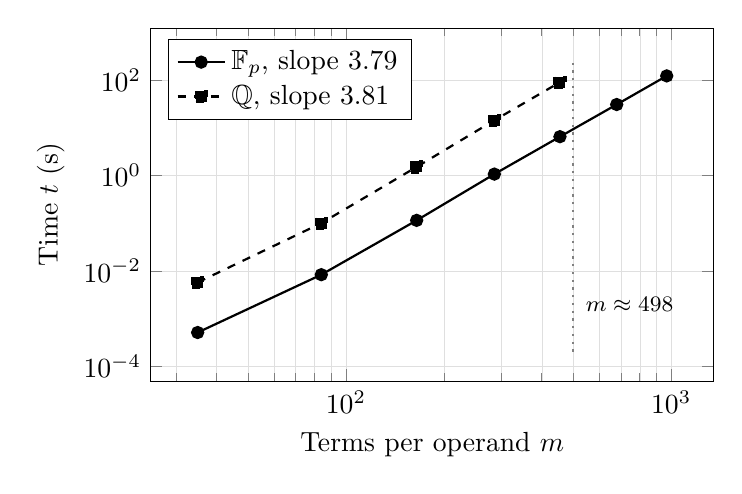
\begin{tikzpicture}
\begin{loglogaxis}[
  width=0.72\textwidth, height=0.5\textwidth,
  xlabel={Terms per operand $m$},
  ylabel={Time $t$ (\si{\second})},
  legend pos=north west,
  legend cell align=left,
  grid=both,
  grid style={line width=0.1pt, draw=gray!25},
  ]
\addplot[mark=*, thick] coordinates {
  (35,0.000505) (84,0.008278) (165,0.114564) (286,1.073065)
  (455,6.554416) (680,31.064855) (969,124.013371)
};
\addlegendentry{$\FF_p$, slope $3.79$}
\addplot[mark=square*, thick, dashed] coordinates {
  (35,0.005692) (84,0.099993) (165,1.519231) (286,14.463953) (455,91.276337)
};
\addlegendentry{$\QQ$, slope $3.81$}
\addplot[dotted, thick, gray, forget plot] coordinates {(498,2e-4) (498,3e2)};
\node[anchor=west, font=\footnotesize] at (axis cs:510,0.002) {$m \approx 498$};
\end{loglogaxis}
\end{tikzpicture}
\caption{Cost of one subresultant gcd against operand size, both axes logarithmic. The two series are
parallel, so the coefficient field contributes a multiplicative constant and not an exponent. The
vertical line marks the operand size observed during the failing three-parameter run, which lies
inside the measured range.}
\label{fig:gcd}
\end{figure}

Fitting $\log t = \alpha \log m + \beta$ by least squares over the points of Table~\ref{tab:gcd}
gives
\[
  \alpha_{\FF_p} = 3.79, \qquad \alpha_{\QQ} = 3.81 .
\]
The ratio $t_{\QQ}/t_{\FF_p}$ rises from $11.3$ at $m = 35$ and settles near $13.9$ at $m = 455$.

\section{Analysis}
\label{sec:analysis}

\subsection{Separation of the two effects}

The controls of Table~\ref{tab:controls} establish that the substitution of $\FF_p$ for $\QQ$
preserves the computation on the two-parameter inputs, by the criterion of Remark~\ref{rem:control}.
The three-parameter system then fails to terminate in a setting where coefficient arithmetic is a
machine-word operation and coefficients do not grow, which is inconsistent with H1 as an explanation
of the failure.

Table~\ref{tab:gcd} quantifies what remains. The two fitted exponents agree to within $0.02$, so the
coefficient field affects the constant $\beta$ and leaves $\alpha$ unchanged; this is visible in
Figure~\ref{fig:gcd} as two parallel lines. The exponent $\alpha \approx 3.8$ is a property of the
subresultant remainder sequence applied to multivariate operands: the sequence performs a number of
pseudo-divisions growing with the degree in the main variable, each pseudo-division is a polynomial
multiplication and exact division on the remaining variables, and the content computations recurse
into those variables in turn~\cite{collins1967,brown1971}. The measured $\alpha$ is consistent with
that structure and is present over both fields.

\subsection{Consequences for modular gcd algorithms}

The term \emph{modular gcd} covers two constructions with different consequences here.

The first computes the same subresultant remainder sequence over several primes and reconstructs the
result by the Chinese remainder theorem, with a trial division to certify the
candidate~\cite{brown1971}. This addresses coefficient growth and leaves the sequence itself intact,
so its benefit is bounded by the ratio measured in Table~\ref{tab:gcd}, namely a factor of
approximately $13$. Applied to a computation that has not completed in \SI{900}{\second}, a factor of
$13$ does not produce a usable result.

The second reduces the multivariate problem to univariate gcds at sampled points and recovers the
answer by interpolation, in the dense form due to Brown~\cite{brown1971} or the sparse form due to
Zippel~\cite{zippel1979}, with the Hensel-based variant of Moses and Yun~\cite{mosesyun1973} a
further alternative. This replaces the remainder sequence and therefore acts on $\alpha$ rather than
on $\beta$. It is the construction that addresses the cost measured here.

\subsection{The operating point}

Interpolating Table~\ref{tab:gcd} between $m = 455$ and $m = 680$ at the exponent $\alpha = 3.79$
places a single gcd at $m = 498$ at approximately \SI{9}{\second} over $\FF_p$ and, applying the
measured ratio, approximately \SI{125}{\second} over $\QQ$. Both figures are consistent with the
intervals between consecutive normalisations reported in Section~\ref{sec:three}. Since $m = 498$
lies inside the range covered by Table~\ref{tab:gcd}, this statement requires no extrapolation.

\section{Threats to validity}
\label{sec:threats}

\paragraph{Necessity without sufficiency.}
The experiment establishes that a faster gcd is necessary for the three-parameter problem. It does
not establish sufficiency. The number of reductions the completion requires is unknown, since the
run has never terminated, and a gcd with a lower exponent would remove the present obstruction
without guaranteeing termination in useful time. Determining the number of reductions would require
either a completed run or an independent bound on the size of the reduced basis over $\QQ(\bp)$.

\paragraph{Density of the benchmark operands.}
The operands of Table~\ref{tab:gcd} are dense of their total degree, whereas the parameter
polynomials arising in the pipeline are not necessarily dense. Density fixes the relation between
degree and term count and makes $m$ an unambiguous size measure, at the cost of favouring dense
interpolation over the sparse method of~\cite{zippel1979} in any comparison of the two. It does not
affect the separation of $\alpha$ from $\beta$, which is the conclusion drawn.

\paragraph{Single prime.}
One prime was used for the substitution. The control of Remark~\ref{rem:control} verifies that it is
not unlucky on the two-parameter inputs, and it cannot be verified on the three-parameter input,
which does not complete. An unlucky prime would be expected to alter the initial ideal and hence the
course of the computation; it would not be expected to convert a terminating computation into a
non-terminating one, since the failure is localised to a single reduction whose operands grow for
reasons independent of the prime.

\paragraph{Timeout as evidence of non-termination.}
The statements that the three-parameter runs do not complete are bounded observations at
\SI{400}{\second} and \SI{900}{\second} rather than proofs of non-termination. The instrumentation of
Section~\ref{sec:three}, showing one pair processed and none thereafter, is the stronger evidence
and is what the analysis relies upon.

\paragraph{Implementation specificity.}
All measurements concern one implementation of Buchberger's algorithm with the normal selection
strategy and grevlex order. A completion algorithm of the F4 family~\cite{faugere1999}, which
replaces sequential reduction by row reduction of a large matrix, would change the number and shape
of the coefficient operations and has not been measured.

\section{Conclusions}
\label{sec:conclusions}

\begin{enumerate}
  \item The three-parameter parametric position problem does not complete over $\FF_p(x,y,z)$ within
        \SI{400}{\second}, so its cost is not attributable to arithmetic on rational coefficients.
        Hypothesis H1 is rejected as an explanation of the limitation.
  \item The subresultant gcd on dense trivariate operands costs $\Theta(m^{\alpha})$ with
        $\alpha \approx 3.8$ measured over both fields, and the coefficient field contributes a
        bounded multiplicative factor of approximately $13$.
  \item The operands reached within one reduction of the three-parameter run number $498$ terms, a
        value interior to the measured range, placing a single gcd at approximately \SI{9}{\second}
        over $\FF_p$.
  \item A modular gcd formed by computing the existing remainder sequence over several primes is
        bounded by the factor of $13$ and would not render the three-parameter problem tractable. A
        gcd based on evaluation and interpolation acts on the exponent and is the construction that
        addresses the measured cost; whether it suffices is not established here.
  \item For the implementation as it stands, $P = 2$ is the working limit, and three-joint arms are
        better obtained by the decoupling of~\cite{pieper1968}, which reduces such an arm to a
        two-parameter problem completed in \SI{25}{\milli\second}.
\end{enumerate}

\appendix

\section{Reproduction}
\label{app:repro}

From the repository root:

\begin{verbatim}
g++ -std=c++17 -O2 doc/experiments/field_cost.cpp -o field_cost \
  -Ivarietas_core/include -Ivarietas_codegen/include \
  -Ivarietas_kinematics/include -Idoc/experiments \
  -I/usr/include/eigen3 -lgmpxx -lgmp

./field_cost planar      # two-parameter control, both fields
./field_cost reduced     # two-parameter control, both fields
./field_cost spatial-fp  # three parameters over F_p; does not terminate
./field_cost spatial-q   # three parameters over Q;   does not terminate

g++ -std=c++17 -O2 doc/experiments/gcd_cost.cpp -o gcd_cost \
  -Ivarietas_core/include -Ivarietas_codegen/include \
  -Idoc/experiments -I/usr/include/eigen3 -lgmpxx -lgmp

./gcd_cost               # Table 2 and the fitted exponents
\end{verbatim}

Adding \texttt{-DVARIETAS\_EXPERIMENT\_TRACE} to the first build reports the largest parameter
polynomial encountered during normalisation, which is the source of the figure $m = 498$. The
pair-queue statistics of Section~\ref{sec:three} were obtained with a temporary instrumented copy of
\texttt{varietas\_core/include/varietas/core/ideal/buchberger.hpp} printing the basis size, the
pending pair count and the largest basis polynomial on each pass through the main loop.

\begin{thebibliography}{99}

\bibitem{arnold2003}
E.~A. Arnold.
\newblock Modular algorithms for computing Gr\"obner bases.
\newblock \emph{Journal of Symbolic Computation}, 35(4):403--419, 2003.

\bibitem{brown1971}
W.~S. Brown.
\newblock On Euclid's algorithm and the computation of polynomial greatest common divisors.
\newblock \emph{Journal of the ACM}, 18(4):478--504, 1971.

\bibitem{buchberger1965}
B.~Buchberger.
\newblock \emph{Ein Algorithmus zum Auffinden der Basiselemente des Restklassenringes nach einem
nulldimensionalen Polynomideal}.
\newblock PhD thesis, University of Innsbruck, 1965.

\bibitem{collins1967}
G.~E. Collins.
\newblock Subresultants and reduced polynomial remainder sequences.
\newblock \emph{Journal of the ACM}, 14(1):128--142, 1967.

\bibitem{coxlittleoshea}
D.~A. Cox, J.~Little, and D.~O'Shea.
\newblock \emph{Ideals, Varieties, and Algorithms}.
\newblock Springer, 4th edition, 2015.

\bibitem{eisenbud}
D.~Eisenbud.
\newblock \emph{Commutative Algebra with a View Toward Algebraic Geometry}.
\newblock Springer, 1995.

\bibitem{faugere1999}
J.-C. Faug\`ere.
\newblock A new efficient algorithm for computing Gr\"obner bases (F4).
\newblock \emph{Journal of Pure and Applied Algebra}, 139(1--3):61--88, 1999.

\bibitem{gathengerhard}
J.~von zur Gathen and J.~Gerhard.
\newblock \emph{Modern Computer Algebra}.
\newblock Cambridge University Press, 3rd edition, 2013.

\bibitem{leeliang1988}
H.-Y. Lee and C.-G. Liang.
\newblock A new vector theory for the analysis of spatial mechanisms.
\newblock \emph{Mechanism and Machine Theory}, 23(3):209--217, 1988.

\bibitem{manochacanny1994}
D.~Manocha and J.~F. Canny.
\newblock Efficient inverse kinematics for general 6R manipulators.
\newblock \emph{IEEE Transactions on Robotics and Automation}, 10(5):648--657, 1994.

\bibitem{moller1995}
H.~M. M\"oller and H.~J. Stetter.
\newblock Multivariate polynomial equations with multiple zeros solved by matrix eigenproblems.
\newblock \emph{Numerische Mathematik}, 70(3):311--329, 1995.

\bibitem{mosesyun1973}
J.~Moses and D.~Y.~Y. Yun.
\newblock The EZ GCD algorithm.
\newblock In \emph{Proceedings of the ACM Annual Conference}, pages 159--166, 1973.

\bibitem{pieper1968}
D.~L. Pieper.
\newblock \emph{The Kinematics of Manipulators under Computer Control}.
\newblock PhD thesis, Stanford University, 1968.

\bibitem{raghavanroth1993}
M.~Raghavan and B.~Roth.
\newblock Inverse kinematics of the general 6R manipulator and related linkages.
\newblock \emph{Journal of Mechanical Design}, 115(3):502--508, 1993.

\bibitem{zippel1979}
R.~Zippel.
\newblock Probabilistic algorithms for sparse polynomials.
\newblock In \emph{Proceedings of EUROSAM '79}, volume 72 of \emph{Lecture Notes in Computer
Science}, pages 216--226. Springer, 1979.

\end{thebibliography}

\end{document}
